\chapter{Технологический раздел}

В данном разделе описаны используемые языки программирования и среда
разработки.

\section{Выбор языка программирования и среды разработки}

Исследование реализаций алгоритмов будет проведено на операционной системе
\text{«Windows»}. Поэтому для создания оконного приложения используется
интерфейс прикладного программирования Win32 API. Это набор функций
для создания программ, работающих под управлением Microsoft Windows 98,
Windows NT или Windows 2000. Все функции этого набора являются 32-битными,
что отражено в названии интерфейса~\cite{Win32Api_Shupak}.

Инициализация, заполнение, обновление и использование теневых карт
предполагается в шейдерных программах. Для этого требуется инициализация
контекста \textit{«OpenGL»} и загрузка необходимых расширений, 
позволяющих компилировать такие программы. Для того,
чтобы связать контекст и оконное приложение на операционной системе
\text{«Windows»} требуется непосредственно сама библиотека
\textit{«opengl32.lib»}~\cite{extOpenGL}.

В ходе разработки реализации алгоритмов теневых карт потребуется
использование матричных преобразований. Они должны не только позволять
производить непосредственно сами преобразования, но и удовлетворять
требованиям использования в шейдерных программах. А именно их представление
в памяти должно соответсвовать ожиданиям шейдеров. Для этого отдельно
разработан модуль линейной алгебры~\cite{Linal}.

Таким образом, в качестве среды программирования выбрана программа
\text{Visual Studio Code}. Основным языком программирования всего приложения
выбран \text{C++}. Для разработки модуля матричных преобразований выбран язык
\text{C}, который наибольшим образом схож с языком программирования шейдерных
программ -- \text{GLSL}.

\section{Выбор графического API}

Для реализации алгоритмов рисования экранируемых и собственных теней в реальном времени
был выбран графический API - OpenGL, предоставляющий работу с графическими
ускорителями (\hbox{рисунок~\ref{img:cpu_gpu_interaction}})~\cite{extOpenGL}.

\begin{figure}[h!]
    \centering
    \includesvg[width=0.8\linewidth]{charts/3dAPImodern.svg}
    \caption{Схема взаимодействия приложения с графическим ускорителем через API.}
    \label{img:cpu_gpu_interaction}
\end{figure}

OpenGL был выбран, исходя из предоставляемых функциональных возможностей
графических API (таблица~\ref{tab:api_comparison}).

\begin{longtable}{|p{4cm}|p{3.8cm}|p{3.8cm}|p{3.8cm}|}
\captionsetup{justification=raggedright,singlelinecheck=false}
\caption{Сравнение графических API} \label{tab:api_comparison} \\

\hline
\textbf{Критерий} & \textbf{OpenGL} & \textbf{Vulkan} & \textbf{DirectX} \\
\hline
\endfirsthead

\hline
\textbf{Критерий} & \textbf{OpenGL} & \textbf{Vulkan} & \textbf{DirectX} \\
\hline
\endhead

\hline
\endfoot

\hline
\textbf{Тип API} & Высокоуровне-вый & Низкоуровне-вый & Высокоуровне-вый \\
\hline
\textbf{Кроссплатфор-менность} & Поддержка Windows, macOS, Linux & Поддержка Windows, Linux, частичная поддержка macOS & Windows \\
\hline
\textbf{Производитель-ность} & Ограничения многопоточности, потеря производительности из -- за высокой нагруженности драйверов & Поддержка многопоточности, эффективное использование ресурсов GPU & Высокая, оптимизация для Windows \\
\hline
\textbf{Поддержка графических возможностей} & Поддержка кадровых буферов (FBO), шейдеров, текстурных массивов & Поддержка многопоточности, полный контроль над ресурсами графических ускорителей & Ограниченные возможности для конкретной платформы \\
\hline

\end{longtable}

В итоге, OpenGL предоставляет весь необходимый функционал,
является кроссплатформенным и высокоуровневым, что позволяет наибольшим
образом сосредоточиться на реализации алгоритмов теней, делегируя прочие задачи
на драйверы графических устройств.

\section{Зависимость компонентов}

На рисунке~\ref{chart:appuml} представлена зависимость компонентов программы.

\begin{figure}[h]
    \centering
    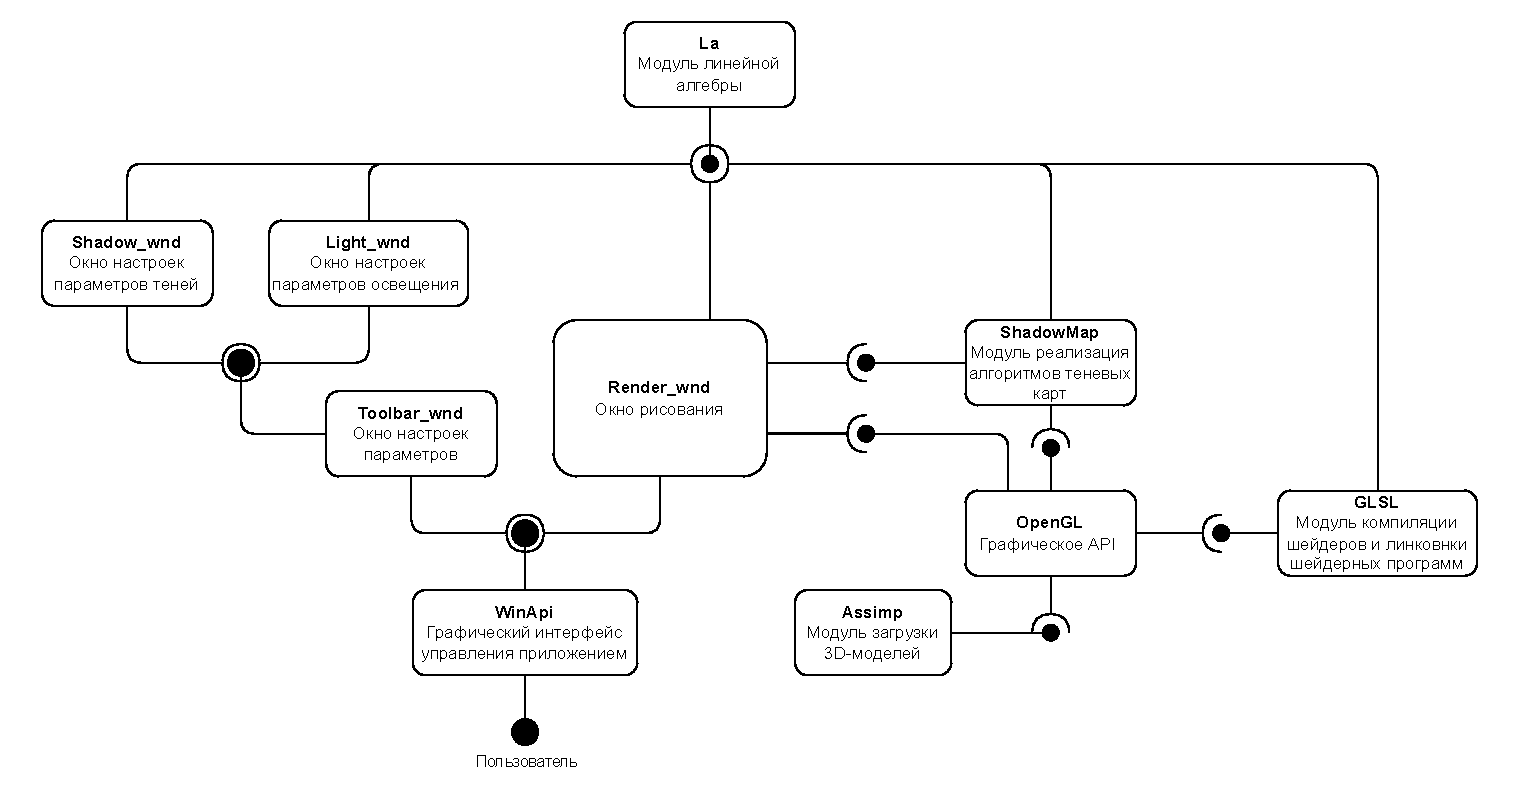
\includegraphics[width=\textwidth]{charts/AppUml.pdf}
    \caption{Диаграмма зависимостей компонентов}
    \label{chart:appuml}
\end{figure}
\FloatBarrier

\section{Исходные модули программы}

Программа для удобства разделена на модули:

\begin{enumerate}[label=\arabic*), labelsep=0.5em]
    \item модуль \text{«LA»} - статическая библиотека линейной алгебры, реализующая
    матричные преобразования, работу с векторами и кватернионами и обеспечивающая
    выравнивание данных в памяти, ожидаемое в шейдерных программах;
    \item модуль \text{«WINAPI»} - статическая библиотека, обеспечивающая создание
    оконного приложения с поддержкой инициализации контекста \textit{«OpenGL»} (версией 4.6)
    и их совместное связывание;
    \item модуль \text{«GLSL»} - статическая библиотека, предоставляющая компилирование, линкование,
    анализ шейдерных программ, оптимизирует рутинные действия при работе с шейдерами;
    \item модуль \text{«ShadowMap»} - статическая библиотека, в которую собраны исследуемые реализации
    алгоритмов теневых карт;
    \item модуль \text{«app»} является основным модулем всего приложения и связывает все
    модули, упомянутые выше, в единое целое.
\end{enumerate}

\subsection{Исходные файлы модуля \text{«LA»}}

В данной библиотеке реализованы такие математические объекты как:

\begin{itemize}[label=---]
    \item вектор с 2-мя компонентами,
    \item вектор с 3-мя компонентами,
    \item вектор с 4-мя компонентами,
    \item кватернион,
    \item матрица размерностью 2 на 2,
    \item матрица размерностью 3 на 3,
    \item матрица размерностью 4 на 4.
\end{itemize}

Файлы модуля представлены ниже:

\begin{itemize}[label=---]
    \item \textbf{заголовочные} файлы:
    \begin{enumerate}[label=\arabic*), labelsep=0.5em]
        \item \text{LA\_sup.h} -- объявление вспомогательных функций для данного модуля;
        \item \text{Matrix2D.h} -- объявление структуры матрицы размерностью 2 на 2 и функций по ее использованию;
        \item \text{Matrix3D.h} -- объявление структуры матрицы размерностью 3 на 3 и функций по ее использованию;
        \item \text{Matrix4D.h} -- объявление структуры матрицы размерностью 4 на 4 и функций по ее использованию;
        \item \text{Quaternion.h} -- объявление структуры кватерниона и функций по его использованию;
        \item \text{Vector2D.h} -- объявление структуры вектора с 2-мя компонентами и функций по его использованию;
        \item \text{Vector3D.h} -- объявление структуры вектора с 3-мя компонентами и функций по его использованию;
        \item \text{Vector4D.h} -- объявление структуры вектора с 4-мя компонентами и функций по его использованию;
    \end{enumerate}
    \item \textbf{исходные} файлы:
    \begin{enumerate}[label=\arabic*), labelsep=0.5em]
        \item \text{LA\_sup.c} -- реализация вспомогательных функций для данного модуля;
        \item \text{Matrix2D.c} -- реализация матричных функций для размерности 2 на 2;
        \item \text{Matrix3D.c} -- реализация матричных функций для размерности 3 на 3;
        \item \text{Matrix4D.c} -- реализация матричных функций для размерности 4 на 4;
        \item \text{Quaternion.c} -- реализация функций преобразований, задаваемых кватернионом;
        \item \text{Vector2D.c} --  реализация функций взаимодействия с 2-ух компонентными векторами;
        \item \text{Vector3D.c} --  реализация функций взаимодействия с 3-ех компонентными векторами;
        \item \text{Vector4D.c} --  реализация функций взаимодействия с 4-ех компонентными векторами;
    \end{enumerate}
\end{itemize}

\subsection{Исходные файлы модуля \text{«WINAPI»}}

Файлы модуля представлены ниже:

\begin{itemize}[label=---]
    \item \textbf{заголовочные} файлы:
    \begin{enumerate}[label=\arabic*), labelsep=0.5em]
        \item \text{winapi\_brush\_struct.h} -- объявление структуры кисти;
        \item \text{winapi\_brash.h} -- объявление класса, реализующего инициализацию, использование и освобождение кисти;
        \item \text{winapi\_char\_converter.h} -- объявление функций конвертации строк;
        \item \text{winapi\_choose\_color\_dialog.h} -- объявление функции вызова диалога выбора цвета;
        \item \text{winapi\_choose\_file\_dialog.h} -- объявление функции вызова диалога выбора файла;
        \item \text{winapi\_common.h} -- объявление вспомогательных функций, специфичных для данного модуля;
        \item \text{winapi\_console.h} -- объявление класса, обеспечивающего создание консоли и перенаправления потоков ввода-вывода;
        \item \text{winapi\_font\_common.h} -- объявление общих функций работы с шрифтами;
        \item \text{winapi\_font\_struct.h} -- объявление структуры шрифта;
        \item \text{winapi\_font.h} -- объявление класса, обеспечивающего создание, использование и освобождение шрифта;
        \item \text{winapi\_GLextensions.h} -- объявление функции загрузки расширений контекста \textit{«OpenGL»};
        \item \text{winapi\_GLwindow.h} -- объявление класса, реализующего создание, использование и освобождение окна, поддерживающего связывание с контекстом \textit{«OpenGL»}; 
        \item \text{winapi\_mat\_ext.h} -- объявление общих расчетных функций, специфичных для данного модуля;
        \item \text{winapi\_mouse.h} -- объявление класса мыши, реализующего взаимодействие с вводом мыши;
        \item \text{winapi\_str\_converter.h} -- объявление расширенных функций конвертации строк;
        \item \text{winapi\_window.h} -- объявление класса, реализующего создание, использование и освобождение окна;
    \end{enumerate}
    \item \textbf{исходные} файлы:
    \begin{enumerate}[label=\arabic*), labelsep=0.5em]
        \item \text{winapi\_brash.cpp} -- реализация класса, обеспечивающего инициализацию, использование и освобождение кисти;
        \item \text{winapi\_char\_converter.cpp} -- реализация функций конвертации строк;
        \item \text{winapi\_choose\_color\_dialog.cpp} -- реализация функции вызова диалога выбора цвета;
        \item \text{winapi\_choose\_file\_dialog.cpp} -- реализация функции вызова диалога выбора файла;
        \item \text{winapi\_common.cpp} -- реализация вспомогательных функций, специфичных для данного модуля;
        \item \text{winapi\_console.cpp} -- реализация класса, обеспечивающего создание консоли и перенаправления потоков ввода-вывода;
        \item \text{winapi\_font\_common.cpp} -- реализация общих функций работы с шрифтами;
        \item \text{winapi\_font.cpp} -- реализация класса, обеспечивающего создание, использование и освобождение шрифта;
        \item \text{winapi\_GLextensions.cpp} -- реализация функции загрузки расширений контекста \textit{«OpenGL»};
        \item \text{winapi\_GLwindow.cpp} -- реализация класса, обеспечивающего создание, использование и освобождение окна, поддерживающего связывание с контекстом \textit{«OpenGL»}; 
        \item \text{winapi\_mat\_ext.cpp} -- реализация общих расчетных функций, специфичных для данного модуля;
        \item \text{winapi\_mouse.cpp} -- реализация класса мыши, обеспечивающего взаимодействие с вводом мыши;
        \item \text{winapi\_str\_converter.cpp} -- реализация расширенных функций конвертации строк;
        \item \text{winapi\_window.cpp} -- реализация класса, обеспечивающего создание, использование и освобождение окна;
    \end{enumerate}
\end{itemize}

\subsection{Исходные файлы модуля \text{«GLSL»}}

Файлы модуля представлены ниже:

\begin{itemize}[label=---]
    \item \textbf{заголовочные} файлы:
    \begin{enumerate}[label=\arabic*), labelsep=0.5em]
        \item \text{shader\_extensions.h} -- объявление функций упрощения отправки данных в шейдерные программы;
        \item \text{shader.h} -- объявление класса, обеспечивающего компилирование, линкование и
        анализ шейдерных программ;
    \end{enumerate}
    \item \textbf{исходные} файлы:
    \begin{enumerate}[label=\arabic*), labelsep=0.5em]
        \item \text{shader\_extensions.cpp} -- реализация функций упрощения отправки данных в шейдерные программы;
        \item \text{shader.cpp} -- реализация класса, обеспечивающего компилирование, линкование и
        анализ шейдерных программ;
    \end{enumerate}
\end{itemize}

\subsection{Исходные файлы модуля \text{«ShadowMap»}}

Файлы модуля представлены ниже:

\begin{itemize}[label=---]
    \item \textbf{заголовочные} файлы:
    \begin{enumerate}[label=\arabic*), labelsep=0.5em]
        \item \text{DepthBufferGenerator.h} -- объявление функции создания теневой карты;
        \item \text{DepthBufferStruct.h} -- объявление структуры теневой карты;
        \item \text{ShadowMapMainRenderData.h} -- объявление структуры необходимых данных для
        стандартного алгоритма теневых карт;
        \item \text{ShadowMapPcfRenderData.h} -- объявление структуры необходимых данных для
        алгоритма теневых карт с фильтрацией (PCF);
        \item \text{ShadowMapNoiseRenderData.h} -- объявление структуры необходимых данных для
        алгоритма теневых карт с фильтрацией шумом (NOISE);
        \item \text{ShadowMapPcssRenderData.h} -- объявление структуры необходимых данных для
        алгоритма мягких теневых карт с фильтрацией (PCSS);
        \item \text{ShadowMapPcssNoiseRenderData.h} -- объявление структуры необходимых данных для
        алгоритма мягких теневых карт с фильтрацией шумом (PCSS-NOISE);
        \item \text{ShadowMap.h} -- объявление функций стандартного алгоритма теневых карт;
        \item \text{ShadowMapPcf.h} -- объявление функций алгоритма теневых карт с фильтрацией (PCF);
        \item \text{ShadowMapNoise.h} -- объявление функций алгоритма теневых карт с фильтрацией шумом (NOISE);
        \item \text{ShadowMapPcss.h} -- объявление функций алгоритма мягких теневых карт с фильтрацией (PCSS);
        \item \text{ShadowMapPcssNosie.h} -- объявление функций алгоритма мягких теневых карт с фильтрацией шумом (PCSS-NOISE);
    \end{enumerate}
    \item \textbf{исходные} файлы:
    \begin{enumerate}[label=\arabic*), labelsep=0.5em]
        \item \text{DepthBufferGenerator.cpp} -- реализация функции создания теневой карты;
        \item \text{ShadowMap.cpp} -- реализация функций стандартного алгоритма теневых карт;
        \item \text{ShadowMapPcf.cpp} -- реализация функций алгоритма теневых карт с фильтрацией (PCF);
        \item \text{ShadowMapNoise.cpp} -- реализация функций алгоритма теневых карт с фильтрацией шумом (NOISE);
        \item \text{ShadowMapPcss.cpp} -- реализация функций алгоритма мягких теневых карт с фильтрацией (PCSS);
        \item \text{ShadowMapPcssNosie.cpp} -- реализация функций алгоритма мягких теневых карт с фильтрацией шумом (PCSS-NOISE);
    \end{enumerate}
\end{itemize}

\subsection{Исходные файлы модуля \text{«app»}}

Файлы модуля представлены ниже:

\begin{itemize}[label=---]
    \item \textbf{заголовочные} файлы:
    \begin{enumerate}[label=\arabic*), labelsep=0.5em]
        \item \text{app\_args.h} -- объявление глобальных переменных приложения;
        \item \text{user\_msgs.h} -- объявление пользовательских событий;
        \item \text{resource.h} -- объявление индетификаторов элементов оконного приложения;
        \item \text{cpu\_stop\_watch.hpp}; -- реализация класса таймера;
        \item \text{cpu\_timing.h} -- объявление базового класса замера процессорного времени;
        \item \text{formater.h} -- объявление функций конвертации строки в число;
        \item \text{FpsSetterDialogProc.h} -- объявление функции обработки событий диалога установки числа обновления кадров в секунду;
        \item \text{general\_shadow\_options\_wnd\_proc.h} -- объявление функции обработки событий окна изменения общих параметров теней;
        \item \text{Light.h} -- объявление функций обновления данных UBO буфера;
        \item \text{lighting\_wnd\_proc.h} -- объявление функции обработки событий окна изменения параметров источника света;
        \item \text{LightStruct.h} -- объявление структуры, описывающей источник света с выравниванием, требуемым шейдерными программами;
        \item \text{main\_wnd\_proc.h} -- объявление функции обработки событий родительского окна;
        \item \text{ModelLoader.h} -- объявление функций загрузки трехмерной модели;
        \item \text{ModelLoaderDialogProc.h} -- объявление функции обработки событий диалога выбора загружаемой модели;
        \item \text{PlaneMeshGenerator.h} -- объявление функций создания специфичных примитивных трехмерных объектов;
        \item \text{ProjectionEnum.h} -- объявление перечисления режима проекции;
        \item \text{render\_wnd\_proc.h} -- объявление функции обработки событий окна отрисовки;
        \item \text{ResolutionMapLimit.h} -- объявление максимальных размеров теневых карт;
        \item \text{shadow\_wnd\_proc.h} -- объявление функции обработки событий окна держателя вкладок;
        \item \text{ShadowAlgEnum.h} -- объявление перечисления алгоритмов теней;
        \item \text{shadowMap\_wnd\_proc.h} -- объявление функции обработки событий окна изменения параметров тени;
        \item \text{time\_definers.h} -- объявление временных констант;
        \item \text{toolbar\_wnd\_proc.h} -- объявление функции обработки событий окна инструментов;
    \end{enumerate}
    \item \textbf{исходные} файлы:
    \begin{enumerate}[label=\arabic*), labelsep=0.5em]
        \item \text{cpu\_timing.cpp} -- реализация базового класса замера процессорного времени;
        \item \text{formater.cpp} -- реализация функций конвертации строки в число;
        \item \text{FpsSetterDialogProc.cpp} -- реализация функции обработки событий диалога установки числа обновления кадров в секунду;
        \item \text{general\_shadow\_options\_wnd\_proc.cpp} -- реализация функции обработки событий окна изменения общих параметров теней;
        \item \text{Light.cpp} -- реализация функций обновления данных UBO буфера;
        \item \text{lighting\_wnd\_proc.cpp} -- реализация функции обработки событий окна изменения параметров источника света;
        \item \text{main\_wnd\_proc.cpp} -- реализация функции обработки событий родительского окна;
        \item \text{main.cpp} -- точка входы программы;
        \item \text{ModelLoader.cpp} -- реализация функций загрузки трехмерной модели;
        \item \text{ModelLoaderDialogProc.cpp} -- реализация функции обработки событий диалога выбора загружаемой модели;
        \item \text{PlaneMeshGenerator.cpp} -- реализация функций создания специфичных примитивных трехмерных объектов;
        \item \text{render\_wnd\_proc.cpp} -- реализация функции обработки событий окна отрисовки;
        \item \text{shadow\_wnd\_proc.cpp} -- реализация функции обработки событий окна держателя вкладок;
        \item \text{shadowMap\_wnd\_proc.cpp} -- реализация функции обработки событий окна изменения параметров тени;
        \item \text{toolbar\_wnd\_proc.cpp} -- реализация функции обработки событий окна инструментов;
    \end{enumerate}
\end{itemize}

\section{Реализация алгоритмов}

В данном разделе будут описаны выбранные типы, структуры данных и
представлены реализации алгоритмов теней.

\subsection{Типы и структуры данных}

В листинге~\ref{lst:light_struct} представлена структура, описывающая источник
освещения в Ламбертовой модели с учетом выравнивания памяти, ожидаемой в шейдерных
программах.

Чтобы передать структуру с ожидаемым расположением полей в структуре в шейдер 
необходимо следовать следующим правилам.

\begin{enumerate}[label=\arabic*), labelsep=0.5em]
    \item Если элемент представляет собой скаляр, использующий \(N\) базовых машинных единиц,
    базовое выравнивание равно \(N\).
    \item Если элемент представляет собой двух- или четырехкомпонентный вектор с компонентами
    при использовании \(N\) базовых машинных единиц базовое выравнивание равно \(2N\) или
    \(4N\) соответственно.
    \item Если элемент представляет собой трехкомпонентный вектор с компонентами, занимающими
    \(N\) базовых машинных единиц, базовое выравнивание равно \(4N\).
    \item Если элемент представляет собой массив скаляров или векторов, базовое выравнивание
    и шаг массива устанавливаются в соответствии с базовым выравниванием отдельного элемента массива
    в соответствии с правилами (1), (2) и (3) и округляются в большую сторону
    к базовому выравниванию четырехкомпонентного вектора. Массив может содержать отступы в начале
    и конце. Базовое смещение элемента, следующего за массивом, округляется в большую сторону
    до следующего значения, кратного базовому выравниванию.
    \item Если элемент представляет собой матрицу, состоящую из \(C\) столбцов и \(R\)
    строк, матрица хранится идентично массиву из \(C\)
    векторов с \(R\) компонентами в каждой строке, согласно правилу (4).
    \item Если элемент является массивом из \(S\) столбцов, то матрица хранится идентично строке векторов-столбцов \(S \times C\) с
    компонентами \(R\) в каждом, согласно правилу (4).
    \item Если элемент представляет собой матрицу, состоящую из \(C\) столбцов и \(R\) строк,
    то матрица сохраняется идентично массиву векторов с \(R\) строками с \(C\) компонентами,
    согласно правилу (4).
    \item Если элемент представляет собой массив из \(S\) матриц, состоящих из \(R\) строк
    и \(С\) столбцов, то матрица сохраняется идентично строке из \(S \times R\)
    векторов с \(C\) компонентами в каждой строке, согласно правилу (4).
    \item Если элемент является структурой, базовое выравнивание структуры равно
    \(N\), где \(N\) - наибольшее базовое значение выравнивания для любого из ее элементов,
    округленное до базового значения выравнивания для четырехкомпонентного вектора. Затем отдельным
    элементам этой подструктуры присваиваются смещения применяя набор правил рекурсивно,
    где базовое смещение первого элемента подструктуры равно выровненному смещению структуры.
    Структура может иметь отступы в конце; базовое смещение элемента, следующего за подструктурой,
    округляется в большую сторону к следующему кратному базовому выравниванию структуры.
    \item Если элемент представляет собой массив из \(S\) структур, элементы
    массива располагаются по порядку в соответствии с правилом (9).
\end{enumerate}

Рациональнее было бы использовать объединение - \text{union}, но GLSL его не
поддерживает~\cite{OpenGL_DevidVolf}.

\begin{center}
\captionsetup{justification=centering, singlelinecheck=off}
\begin{lstlisting}[label=lst:light_struct, caption={Источник освещения}]
struct Light
{
    // Кратность 16 ==================================================================
    vec3 position;     // Позиция (12 байт)
    float pad0;        // Выравнивание для GLSL vec3 (еще 4 байта)
    // Кратность 16 ==================================================================
    vec3 direction;    // Направление (12 байт)
    float pad1;        // Выравнивание для GLSL vec3 (еще 4 байта)
    // Кратность 16 ==================================================================
    vec3 color;        // Цвет (12 байт)
    float pad2;        // Выравнивание для GLSL vec3 (еще 4 байта)
    // Кратность 16 ==================================================================
    float radius;      // Радиус действия (4 байта)
    float intensity;   // Интенсивность (4 байта)
    float innerCutoff; // Угол (в радианах) внутреннего конуса (4 байта)
    float outerCutoff; // Угол (в радианах) внешнего конуса (4 байта)
    // Кратность 16 ==================================================================
    int   type;        // Тип источника света: 0 - PointLight; 1 - SpotLight (4 байта)
    float pad3;        // Дополнительные паддинги,
    float pad4;        // чтобы сделать размер структуры
    float pad5;        // кратным 16 (3 * 4 = 12 байт)
    // Кратность 16 ==================================================================
};
\end{lstlisting}
\end{center}

В листинге~\ref{lst:shadow_map_main_struct} представлена структура,
описывающая необходимые данные для алгоритма стандартных теневых карт.

\begin{center}
\captionsetup{justification=centering, singlelinecheck=off}
\begin{lstlisting}[label=lst:shadow_map_main_struct, caption={Структура параметров для стандартного алгоритма теневых карт}]
struct ShadowMapMainRenderData
{
    DepthBuffer* depthBuffer; // Структура теневой карты
    GLsizei* client_width;    // Ширина клиентской области рисования в пикселях
    GLsizei* client_height;   // Высота клиентской области рисования в пикселях

    Shader* shaderDepthPass;  // Объект класса шейдер
    Shader* shaderRenderPass; // Объект класса шейдер
    Shader* shaderDepthDebug; // Объект класса шейдер

    mat4* view;               // Матрица вида камеры пользователя
    mat4* projection;         // Матрица проекции камеры пользователя

    mat4* lightView;          // Матрица вида источника освещения
    mat4* lightProjection;    // Матрица проекции источника освещения

    GLfloat* shadowBias;      // Корректирующее смещение

    GLuint* quadVAO;          // Идентификатор буфера двумерного объекта, прямоугольник

    GLuint* planeVAO;         // Идентификатор буфера трехмерного объекта, плоскость
    mat4* planeModel;         // Матрица модели этого объекта

    GLuint* modelVAO;         // Идентификатор буфера трехмерного объекта
    GLsizei* modelIndexCount; // Количество индексов в этой модели
    mat4* modelModel;         // Матрица модели этого объекта
};
\end{lstlisting}
\end{center}

Для всех остальных алгоритмов теневых карт, помимо параметров
приведенных выше, требуется еще один параметр - \text{pcfRadius}.
Таким образом, структура выглядит как в
листинге~\ref{lst:shadow_map_pcf_struct}.

\begin{center}
\captionsetup{justification=centering, singlelinecheck=off}
\begin{lstlisting}[label=lst:shadow_map_pcf_struct, caption={Структура параметров для алгоритмов теневых карт с фильтрацией}]
struct ShadowMapMainRenderData
{
    DepthBuffer* depthBuffer; // Структура теневой карты
    GLsizei* client_width;    // Ширина клиентской области рисования в пикселях
    GLsizei* client_height;   // Высота клиентской области рисования в пикселях

    Shader* shaderDepthPass;  // Объект класса шейдер
    Shader* shaderRenderPass; // Объект класса шейдер
    Shader* shaderDepthDebug; // Объект класса шейдер

    mat4* view;               // Матрица вида камеры пользователя
    mat4* projection;         // Матрица проекции камеры пользователя

    mat4* lightView;          // Матрица вида источника освещения
    mat4* lightProjection;    // Матрица проекции источника освещения

    GLfloat* shadowBias;      // Корректирующее смещение
    GLfloat* pcfRadius;       // Радиус фильтрации

    GLuint* quadVAO;          // Идентификатор буфера двумерного объекта, прямоугольник

    GLuint* planeVAO;         // Идентификатор буфера трехмерного объекта, плоскость
    mat4* planeModel;         // Матрица модели этого объекта

    GLuint* modelVAO;         // Идентификатор буфера трехмерного объекта
    GLsizei* modelIndexCount; // Количество индексов в этой модели
    mat4* modelModel;         // Матрица модели этого объекта
};
\end{lstlisting}
\end{center}

В листингах~\ref{lst:shadow_map_main_struct}~--~\ref{lst:shadow_map_pcf_struct}
использовалась структура \text{теневой карты}. Она описана в
листинге~\ref{lst:shadow_map}.

\begin{center}
\captionsetup{justification=centering, singlelinecheck=off}
\begin{lstlisting}[label=lst:shadow_map, caption={Структура теневой карты}]
struct DepthBuffer
{
    GLuint Texture; // Идентификатор карты - текстуры
    GLuint FBO;     // Идентификатор кадрового буфера
    GLsizei width;  // Длина карты в пикселях
    GLsizei height; // Высота карты в пикселях
};
\end{lstlisting}
\end{center}

\subsection{Реализация основных этапов алгоритмов теней}

Все описанные алгоритмы, как представлено в
схемах~\ref{chart:shadow_map}~--~\ref{chart:shadow_map_pcss_noise},
имеют идентичный этап заполнения карты теней (листинг~\ref{lst:shadow_map_init}).
В этом участке кода, выполняется заполнение теневой карты, в которую заносится
информация глубины объекта.

\begin{center}
\captionsetup{justification=centering, singlelinecheck=off}
\begin{lstlisting}[label=lst:shadow_map_init, caption=Алгоритм заполнения теневой карты]
void DepthPass(ShadowMapMainRenderData& data)
{
    glViewport(0, 0, data.depthBuffer->width, data.depthBuffer->height);

    glBindFramebuffer(GL_FRAMEBUFFER, data.depthBuffer->FBO);
    glClear(GL_DEPTH_BUFFER_BIT);

    data.shaderDepthPass->use();
    uniform_matrix4f(data.shaderDepthPass->get_uniform_location("view"), data.lightView);
    uniform_matrix4f(data.shaderDepthPass->get_uniform_location("projection"), data.lightProjection);

    glBindVertexArray(*data.modelVAO);
    uniform_matrix4f(data.shaderDepthPass->get_uniform_location("model"), data.modelModel);
    glDrawElements(GL_TRIANGLES, *data.modelIndexCount, GL_UNSIGNED_INT, 0);
    glBindVertexArray(0);
}
\end{lstlisting}
\end{center}

Приведенная выше реализация алгоритма заполнения теневой карты, является универсальной для
всех алгоритмов теней, за исключением того, что для каждого алгоритма используется
своя структура данных.

Второй этап алгоритмов теневых карт так же является практически одинаковым для всех реализаций
алгоритмов за исключением передачи некоторых уникальных данных в соответствующую шейдерную
программу. В листинге~\ref{lst:shadow_map_render} приведена реализация этапа рисования сцены с учетом теней для
алгоритма стандартных теневых карт.

\begin{center}
\captionsetup{justification=centering, singlelinecheck=off}
\begin{lstlisting}[label=lst:shadow_map_render, caption=Алгоритм заполнения теневой карты]
void RenderPass(ShadowMapMainRenderData& data)
{
    glViewport(0, 0, *data.client_width, *data.client_height);

    glBindFramebuffer(GL_FRAMEBUFFER, 0);
    glClear(GL_COLOR_BUFFER_BIT | GL_DEPTH_BUFFER_BIT);

    data.shaderRenderPass->use();
    uniform_matrix4f(data.shaderRenderPass->get_uniform_location("view"), data.view);
    uniform_matrix4f(data.shaderRenderPass->get_uniform_location("projection"), data.projection);
    uniform_matrix4f(data.shaderRenderPass->get_uniform_location("lightView"), data.lightView);
    uniform_matrix4f(data.shaderRenderPass->get_uniform_location("lightProjection"), data.lightProjection);
    glUniform1f(data.shaderRenderPass->get_uniform_location("shadowBias"), *data.shadowBias);

    glActiveTexture(GL_TEXTURE0);
    glBindTexture(GL_TEXTURE_2D, data.depthBuffer->Texture);

    glBindVertexArray(*data.modelVAO);
    uniform_matrix4f(data.shaderRenderPass->get_uniform_location("model"), data.modelModel);
    glDrawElements(GL_TRIANGLES, *data.modelIndexCount, GL_UNSIGNED_INT, 0);

    glBindVertexArray(*data.planeVAO);
    uniform_matrix4f(data.shaderRenderPass->get_uniform_location("model"), data.planeModel);
    glDrawElements(GL_TRIANGLES, 6, GL_UNSIGNED_INT, 0);

    glBindVertexArray(0);
}
\end{lstlisting}
\end{center}

Помимо таких параметров как \text{view},
\text{projection}, \text{lightView}, \text{lightProjection} и
\text{shadowBias}, которые являются общими для всех реализаций,
есть дополнительный -- \text{pcfRadius}, используемый во всех
алгоритмах кроме стандартного.

\subsection{Реализация алгоритма стандартных теневых карт}

\subsection*{Подготовительный этап}

В подготовительном этапе рисования теней, представленном в листинге~\ref{lst:shadow_map_init},
используется шейдерная программа, контролирующая заполнение теневой карты значениями глубины
(\hbox{листинги~\ref{lst:shadow_map_init_vert}~--~\ref{lst:shadow_map_init_frag}}).

\begin{center}
\captionsetup{justification=centering, singlelinecheck=off}
\begin{lstlisting}[label=lst:shadow_map_init_vert, caption=Вершинный шейдер заполнения теневой карты]
#version 460 core

layout(location = 0) in vec3 aPos;

uniform mat4 model;
uniform mat4 view;
uniform mat4 projection;

void main()
{
    gl_Position = projection * view * model * vec4(aPos, 1.0);
}
\end{lstlisting}
\end{center}

\begin{center}
\captionsetup{justification=centering, singlelinecheck=off}
\begin{lstlisting}[label=lst:shadow_map_init_frag, caption=Фрагментный шейдер заполнения теневой карты]
#version 460 core

void main()
{

}
\end{lstlisting}
\end{center}

Особенностью реализации фрагментного шейдера (листинг~\ref{lst:shadow_map_init_frag})
является пустая головная функция, так как никакой обработки пикселей не происходит,
за исключением записи значений их глубины в теневую карту, предварительно
подключенную на запись перед рисованием объектов, отбрасывающих тени.

Важно отметить, что рисовать все объекты подряд не требуется. Если достоверно известно,
что экранируемая и собственная тени какого-либо объекта не будут видны с точки зрения пользователя,
то такие объекты можно пропустить. При этом экранируемые тени от других объектов все еще будут корректно
отображаться на поверхностях чужих объектов.

Именно поэтому в подготовительном этапе отображается только обозреваемый объект, в то время как
рисование плоскости игнорируется.

Реализация шейдерной программы, приведенной в
листингах~\ref{lst:shadow_map_init_vert}~--~\ref{lst:shadow_map_init_frag},
является общей для всех реализаций подготовительного этапа рисования теней.

\subsection*{Заключительный этап}

Используя заполненную теневую карту в первом этапе рисования,
заключительная шейдерная программа рисует сцену с учетом теней и освещения
(листинги~\ref{lst:shadow_map_vert}~--~\ref{lst:shadow_map_frag}).

\begin{center}
\captionsetup{justification=centering, singlelinecheck=off}
\begin{lstlisting}[label=lst:shadow_map_vert, caption=Вершинный шейдер преобразования координат]
#version 460 core

layout(location = 0) in vec3 aPos;
layout(location = 1) in vec3 aNormal;

uniform mat4 model;
uniform mat4 view;
uniform mat4 projection;

uniform mat4 lightView;
uniform mat4 lightProjection;

out vec4 FragPos;
out vec3 Normal;
out vec4 FragPosLightSpace;

void main()
{
    FragPos = model * vec4(aPos, 1.0);
    Normal = mat3(transpose(inverse(model))) * aNormal;
    FragPosLightSpace = lightProjection * lightView * FragPos;
    gl_Position = projection * view * FragPos;
}
\end{lstlisting}
\end{center}

\begin{center}
\captionsetup{justification=centering, singlelinecheck=off}
\begin{lstlisting}[label=lst:shadow_map_frag, caption=Фрагментный шейдер с учетом теней и освещения]
#version 460 core

// Определение структур, описывающих освещение ...

out vec4 FragColor;

in vec4 FragPos;
in vec3 Normal;
in vec4 FragPosLightSpace;

uniform sampler2D shadowMap;
uniform float shadowBias;

// Объявление и реализация функций вычисляющих освещение ...

float ShadowCalculation(vec4 fragPosLightSpace)
{
    // Конвертация из [-1, 1] в [0, 1]
    vec3 projCoords = fragPosLightSpace.xyz / fragPosLightSpace.w;
    projCoords = projCoords * 0.5 + 0.5;

    // Глубина текущего фрагмента из карты теней
    float closestDepth = texture(shadowMap, projCoords.xy).r; 
    float currentDepth = projCoords.z;

    // Проверка на тень
    float shadow = step(closestDepth + shadowBias, currentDepth);
    shadow *= step(currentDepth, 1.0);

    return shadow;
}

void main()
{
    vec3 color = vec3(0.5);
    vec3 ambient = 0.15 * color;

    vec3 diffuse = computeLightColor(FragPos.xyz, Normal) * color;

    float shadow = ShadowCalculation(FragPosLightSpace);                      
    vec3 lighting = (ambient + (1.0 - shadow) * diffuse);

    FragColor = vec4(lighting, 1.0);
}
\end{lstlisting}
\end{center}

Вершинный шейдер, представленный в листинге~\ref{lst:shadow_map_vert}
является общим для всех алгоритмов рисования теней.

Фрагментный шейдер (листинг~\ref{lst:shadow_map_frag}) имеет вариацию в зависимости
от вида проецирования: ортогонального или перспективного. В приведенном примере используется
перспективное проецирование тени. Отличие ортогонального проецирования от перспективного
заключается лишь в конвертации координат, то есть измена только функция
\textit{ShadowCalculation()}. Реализация такой вариации приведена в
листинге~\ref{lst:shadow_map_frag_ortho}.

\begin{center}
\captionsetup{justification=centering, singlelinecheck=off}
\begin{lstlisting}[label=lst:shadow_map_frag_ortho, caption=Фрагментный шейдер с учетом ортогонального проецирония теней]
// ...

float ShadowCalculation(vec4 fragPosLightSpace)
{
    // Конвертация из [-1, 1] в [0, 1]
    vec3 projCoords = fragPosLightSpace.xyz;
    projCoords = projCoords * 0.5 + 0.5;

    // Глубина текущего фрагмента из карты теней
    float closestDepth = texture(shadowMap, projCoords.xy).r; 
    float currentDepth = projCoords.z;

    // Проверка на тень
    float shadow = step(closestDepth + shadowBias, currentDepth);
    shadow *= step(currentDepth, 1.0);

    return shadow;
}

//...
\end{lstlisting}
\end{center}

По итогу, перспективное деление игнорируется в силу того, что используется
матрица ортогонального проецирования вместо перспективного.

\subsection{Реализация алгоритма теневых карт с фильтрацией}

Как было уточнено выше, шейдерная программа
(листинги~\ref{lst:shadow_map_init_vert}~--~\ref{lst:shadow_map_init_frag})
в подготовительном этапе эквивалентна во всех реализациях,
так же как и вершинный шейдер в заключительном этапе
(листинг~\ref{lst:shadow_map_vert}). Поэтому здесь и далее для всех
реализаций алгоритмов теней будут приведены только фрагметные шейдеры
заключительного этапа.

В листинге~\ref{lst:shadow_map_pcf_frag} представлена реализация фрагментного шейдера заключительного
этапа рисования с учетом перспективной проекции теней с фильтрацией и освещения.

\begin{center}
\captionsetup{justification=centering, singlelinecheck=off}
\begin{lstlisting}[label=lst:shadow_map_pcf_frag, caption=Фрагментный шейдер с учетом перспективного проецирония теней]
#version 460 core

// Определение структур, описывающих освещение ...

out vec4 FragColor;

in vec4 FragPos;
in vec3 Normal;
in vec4 FragPosLightSpace;

uniform sampler2D shadowMap;
uniform float shadowBias;
uniform float pcfRadius;

// Объявление и реализация функций вычисляющих освещение ...

float ShadowCalculation(vec4 fragPosLightSpace)
{
    // Конвертация из [-1, 1] в [0, 1]
    vec3 projCoords = fragPosLightSpace.xyz / fragPosLightSpace.w;
    projCoords = projCoords * 0.5 + 0.5;

    // Проверка на тень
    if (projCoords.z > 1.0)
        return 0.0;
    
    // Тень с использованием PCF
    float shadow = 0.0;
    vec2 texelSize = 1.0 / textureSize(shadowMap, 0);
    for (int x = -1; x <= 1; ++x)
    {
        for (int y = -1; y <= 1; ++y)
        {
            float pcfDepth = texture(shadowMap, projCoords.xy + vec2(x, y) * texelSize * pcfRadius).r;
            shadow += projCoords.z - shadowBias > pcfDepth ? 1.0 : 0.0;
        }
    }

    return shadow / 9.0;
}

void main()
{
    vec3 color = vec3(0.5);
    vec3 ambient = 0.15 * color;

    vec3 diffuse = computeLightColor(FragPos.xyz, Normal) * color;

    float shadow = ShadowCalculation(FragPosLightSpace);                      
    vec3 lighting = (ambient + (1.0 - shadow) * diffuse);

    FragColor = vec4(lighting, 1.0);
}
\end{lstlisting}
\end{center}

Вариация реализации фрагментного шейдера рисования теней с
фильтрацией с ортогональной проекцией теней представлена в
листинге~\ref{lst:shadow_map_pcf_ortho_frag}, конфигурация которой
заключается только в функции \textit{ShadowCalculation()}.

\begin{center}
\captionsetup{justification=centering, singlelinecheck=off}
\begin{lstlisting}[label=lst:shadow_map_pcf_ortho_frag, caption=Фрагментный шейдер с учетом ортогонального проецирония теней]
// ...

float ShadowCalculation(vec4 fragPosLightSpace)
{
    // Конвертация из [-1, 1] в [0, 1]
    vec3 projCoords = fragPosLightSpace.xyz;
    projCoords = projCoords * 0.5 + 0.5;
    
    // Тень с использованием PCF
    float shadow = 0.0;
    vec2 texelSize = 1.0 / textureSize(shadowMap, 0);
    for (int x = -1; x <= 1; ++x)
    {
        for (int y = -1; y <= 1; ++y)
        {
            float pcfDepth = texture(shadowMap, projCoords.xy + vec2(x, y) * texelSize * pcfRadius).r;
            shadow += projCoords.z - shadowBias > pcfDepth ? 1.0 : 0.0;
        }
    }

    return shadow / 9.0;
}

// ...
\end{lstlisting}
\end{center}

\subsection{Реализация алгоритма теневых карт с фильтрацией шумом}

В листинге~\ref{lst:shadow_map_noise_frag} представлена реализация фрагментного шейдера заключительного
этапа рисования с учетом перспективной проекции теней с фильтрацией шумом и освещения.

\begin{center}
\captionsetup{justification=centering, singlelinecheck=off}
\begin{lstlisting}[label=lst:shadow_map_noise_frag, caption=Фрагментный шейдер с учетом перспективного проецирония теней]
#version 460 core

// Объявление структур, описывающих освещение ...

out vec4 FragColor;

in vec4 FragPos;
in vec3 Normal;
in vec4 FragPosLightSpace;

uniform sampler2D shadowMap;
uniform float shadowBias;
uniform float pcfRadius;

#define PI 3.14159265358

// Объявление и реализация функций вычисляющих освещение ...

// Случайное число
float rand(vec2 uv)
{
    return fract(sin(dot(uv, vec2(12.9898, 4.1414))) * 43758.5453);
}

// Случайное гауссово распределение
float randomGaussian(float mean, float stddev, vec2 seed) {
    float u1 = rand(seed);
    float u2 = rand(seed + vec2(1.0));
    float r = sqrt(-2.0 * log(u1)) * cos(2.0 * PI * u2);
    return mean + stddev * r;
}

// Шум
vec2 generateNoise(float mean, float stddev, vec2 seed)
{
    return vec2(randomGaussian(mean, stddev, seed * PI), randomGaussian(mean, stddev, seed));
}

float ShadowCalculation(vec4 fragPosLightSpace)
{
    // Конвертация из [-1, 1] в [0, 1]
    vec3 projCoords = fragPosLightSpace.xyz / fragPosLightSpace.w;
    projCoords = projCoords * 0.5 + 0.5;

    // Проверка на тень
    if (projCoords.z > 1.0)
        return 0.0;
    
    // Тень с использованием Шума
    float shadow = 0.0;
    vec2 texelSize = 1.0 / textureSize(shadowMap, 0);
    for (int x = -1; x <= 1; ++x)
    {
        for (int y = -1; y <= 1; ++y)
        {
            vec2 noiseOffset = generateNoise(0.0, 1.0, projCoords.xy + vec2(x, y));
            float pcfDepth = texture(shadowMap, projCoords.xy + noiseOffset * texelSize * pcfRadius).r;
            shadow += projCoords.z - shadowBias > pcfDepth ? 1.0 : 0.0;
        }
    }

    return shadow / 9.0;
}

void main()
{
    vec3 color = vec3(0.5);
    vec3 ambient = 0.15 * color;

    vec3 diffuse = computeLightColor(FragPos.xyz, Normal) * color;

    float shadow = ShadowCalculation(FragPosLightSpace);                      
    vec3 lighting = (ambient + (1.0 - shadow) * diffuse);

    FragColor = vec4(lighting, 1.0);
}
\end{lstlisting}
\end{center}

Вариация реализации фрагментного шейдера рисования теней с
фильтрацией шумом с ортогональной проекцией теней представлена в
листинге~\ref{lst:shadow_map_noise_ortho_frag}, конфигурация которой
заключается только в функции \textit{ShadowCalculation()}.

\begin{center}
\captionsetup{justification=centering, singlelinecheck=off}
\begin{lstlisting}[label=lst:shadow_map_noise_ortho_frag, caption=Фрагментный шейдер с учетом ортогонального проецирония теней]
// ...

float ShadowCalculation(vec4 fragPosLightSpace)
{
    // Конвертация из [-1, 1] в [0, 1]
    vec3 projCoords = fragPosLightSpace.xyz;
    projCoords = projCoords * 0.5 + 0.5;

    // Проверка на тень
    if (projCoords.z > 1.0)
        return 0.0;
    
    // Тень с использованием Шума
    float shadow = 0.0;
    vec2 texelSize = 1.0 / textureSize(shadowMap, 0);
    for (int x = -1; x <= 1; ++x)
    {
        for (int y = -1; y <= 1; ++y)
        {
            vec2 noiseOffset = generateNoise(0.0, 1.0, projCoords.xy + vec2(x, y));
            float pcfDepth = texture(shadowMap, projCoords.xy + noiseOffset * texelSize * pcfRadius).r;
            shadow += projCoords.z - shadowBias > pcfDepth ? 1.0 : 0.0;
        }
    }

    return shadow / 9.0;
}

// ...
\end{lstlisting}
\end{center}

\subsection{Реализация алгоритма мягких теневых карт с фильтрацией}

В листинге~\ref{lst:shadow_map_pcss_frag} представлена реализация фрагментного шейдера заключительного
этапа рисования с учетом перспективной проекции мягких теней с фильтрацией и освещения.

\begin{center}
\captionsetup{justification=centering, singlelinecheck=off}
\begin{lstlisting}[label=lst:shadow_map_pcss_frag, caption=Фрагментный шейдер с учетом перспективного проецирония теней]
#version 460 core

// Объявление структур, описывающих освещение ...

out vec4 FragColor;

in vec4 FragPos;
in vec3 Normal;
in vec4 FragPosLightSpace;

in vec2 lightProjectionParams;

uniform sampler2D shadowMap;
uniform float shadowBias;
uniform float pcfRadius;
uniform float lightRadius = 1.0; // Радиус источника света

#define PI 3.14159265358

// Объявление и реализация функций вычисляющих освещение ...

vec2 sampleDisk(int sampleIndex, int numSamples)
{
    float angle = float(sampleIndex) / float(numSamples) * 2.0 * PI;
    return vec2(cos(angle), sin(angle));
}

float SearchBlocker(vec3 projCoords, float searchRadius)
{
    int numSamples = 16;  // количество выборок вокруг текущего фрагмента
    float blockerDepthSum = 0.0;
    int numBlockers = 0;

    // Вычисление размера текстеля
    vec2 texelSize = 1.0 / textureSize(shadowMap, 0); // 0 - уровень MIP карты

    // Выборки вокруг текущей точки (в пределах searchRadius)
    for (int i = 0; i < numSamples; ++i)
    {
        // Генерация смещенной позиции выборки (например, случайное смещение или с использованием диска)
        vec2 offset = sampleDisk(i, numSamples) * texelSize * searchRadius;

        // Чтение глубины из карты теней для соседней точки
        float depthInShadowMap = texture(shadowMap, projCoords.xy + offset).r;

        // Если точка блокирует свет, добавить её глубину
        if (depthInShadowMap < projCoords.z + shadowBias)
        {
            blockerDepthSum += depthInShadowMap;
            ++numBlockers;
        }
    }

    // Если найдены блокирующие объекты, усреднить их глубину
    if (numBlockers > 0)
    {
        return blockerDepthSum / float(numBlockers);
    }

    // Если блокирующие объекты не найдены, вернуть -1
    return -1.0;
}

float EstimatePenumbraSize(float fragDepth, float blockerDepth)
{
    // Если нет блокирующего объекта, полутени нет
    if (blockerDepth < 0.0)
    {
        return 0.0;
    }

    float viewLightFragDepth = lightProjectionParams.y / (fragDepth * 2.0 - 1.0 - lightProjectionParams.x);
    float viewLightBlockerDepth = lightProjectionParams.y / (blockerDepth * 2.0 - 1.0 - lightProjectionParams.x);

    // Оценка размера полутени
    float penumbraSize = (viewLightFragDepth - viewLightBlockerDepth) / viewLightBlockerDepth * lightRadius;

    return penumbraSize;
}

float PerformPCF(vec3 projCoords, float penumbraSize)
{
    // Определение ядра для PCF
    int samleSize = 16; // Предпочтительно нечетное
    int halfSize = samleSize / 2;
    float samleCount = pow(halfSize * 2 + 1, 2.0);

    float shadow = 0.0;
    
    // Применить значение penumbraSize для масштабирования области выборки
    float filterRadius = penumbraSize;

    // Вычисление размера текстеля
    vec2 texelSize = 1.0 / textureSize(shadowMap, 0); // 0 - уровень MIP карты

    // Цикл по выборкам вокруг текущей координаты в пространстве света
    for (int x = -halfSize; x <= halfSize; ++x)
    {
        for (int y = -halfSize; y <= halfSize; ++y)
        {
            float pcfDepth = texture(shadowMap, projCoords.xy + vec2(x, y) * texelSize * filterRadius).r;
            shadow += projCoords.z - shadowBias > pcfDepth ? 1.0 : 0.0;
        }
    }

    return shadow / samleCount;
}

float ShadowCalculation(vec4 fragPosLightSpace)
{
    // Преобразование координат в проекционные
    vec3 projCoords = fragPosLightSpace.xyz / fragPosLightSpace.w;
    projCoords = projCoords * 0.5 + 0.5;

    if (projCoords.z > 1.0)
        return 0.0;

    // Шаг 1: Оценка блокирующих объектов
    float blockerDepth = SearchBlocker(projCoords, pcfRadius);

    if (blockerDepth < 0.0)
        return 0.0;

    // Шаг 2: Оценка размера полутени
    float penumbraSize = EstimatePenumbraSize(projCoords.z, blockerDepth);

    // Шаг 3: Применение PCF с изменяемым радиусом
    return PerformPCF(projCoords, penumbraSize);
}

void main()
{
    vec3 color = vec3(0.5);
    vec3 ambient = 0.15 * color;

    vec3 diffuse = computeLightColor(FragPos.xyz, Normal) * color;

    float shadow = ShadowCalculation(FragPosLightSpace);                      
    vec3 lighting = (ambient + (1.0 - shadow) * diffuse);

    FragColor = vec4(lighting, 1.0);
}
\end{lstlisting}
\end{center}

Вариация реализации фрагментного шейдера рисования мягких теней с
фильтрацией с ортогональной проекцией теней представлена в
листинге~\ref{lst:shadow_map_pcss_ortho_frag}, конфигурация которой
заключается только в функции \textit{ShadowCalculation()}.

\begin{center}
\captionsetup{justification=centering, singlelinecheck=off}
\begin{lstlisting}[label=lst:shadow_map_pcss_ortho_frag, caption=Фрагментный шейдер с учетом ортогонального проецирония теней]
// ...



// ...
\end{lstlisting}
\end{center}
    

\subsection{Реализация алгоритма мягких теневых карт с фильтрацией шумом}

В листинге~\ref{lst:} представлена реализация фрагментного шейдера заключительного
этапа рисования с учетом перспективной проекции мягких теней с фильтрацией шумом и освещения.

Вариация реализации фрагментного шейдера рисования мягких теней с
фильтрацией шумом с ортогональной проекцией теней представлена в
листинге~\ref{lst:}, конфигурация которой
заключается только в функции \textit{ShadowCalculation()}.

\subsection{Реализация алгоритма освещения}

В каждых из выше

\section*{Вывод}